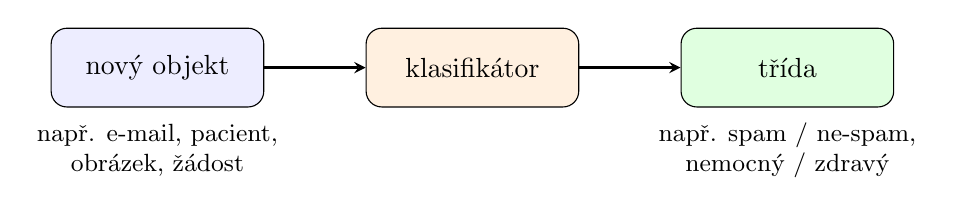
\begin{tikzpicture}[
    >=stealth,
    box/.style={
        draw,
        rounded corners=2mm,
        minimum width=27mm,
        minimum height=10mm,
        align=center,
        fill=blue!7
    },
    arr/.style={->, thick}
]
    \node[box] (obj) at (0,0) {nový objekt};
    \node[box, fill=orange!12] (model) at (4,0) {klasifikátor};
    \node[box, fill=green!12] (cls) at (8,0) {třída};

    \draw[arr] (obj) -- (model);
    \draw[arr] (model) -- (cls);

    \node[align=center, font=\small] at (0,-1.05)
        {např. e-mail, pacient,\\ obrázek, žádost};
    \node[align=center, font=\small] at (8,-1.05)
        {např. spam / ne-spam,\\ nemocný / zdravý};
\end{tikzpicture}
